\subsection{Sensitivity analysis}
\begin{frame}
    \frametitle{Sensitivity analysis provides more insight into 
    the fuel cycles.}
    To meet the third objective, I performed sensitivity analysis 
    on Scenario 7 (once-through, no growth, Xe-100 + VOYGR + MMR), 
    comparing the impact of different model parameters
    \begin{itemize}
        \item Couple \Cyclus with Dakota \cite{adams_dakota_2021}
        \item<2-> Input parameters include:
        \begin{itemize}
            \item<2-> Transition start time
            \item<2-> Percent of \glspl{LWR} operating for 80 years
            \item<2-> Build share of Xe-100, VOYGR, MMR
            \item<2-> Discharge burnup of Xe-100 and MMR
        \end{itemize}
        \item<3-> Output metrics include:
        \begin{itemize}
            \item<3-> Total enriched uranium mass
            \item<3-> HALEU mass
            \item<3-> Total SWU capacity
            \item<3-> SWU capacity to produce HALEU
            \item<3-> Feed uranium to produce HALEU
            \item<3-> \gls{SNF} mass
        \end{itemize}
        \item<4-> Varied parameters individually and multiple combinations
        \item<4-> Modify deployment scheme to prioritize reactor with 
              specified build share, then deploy others in the same 
              manner as before
    \end{itemize}

\end{frame}

\begin{frame}
    \frametitle{Increasing MMR build share increases all metrics}
    \begin{columns}

        \column[t]{4.5cm}
        \begin{itemize}
            \item All of the materials increase
            \item Enrichment-related metrics increase the most
            \item<2-> Results are a function of the number of
                  each advanced reactor deployed
        \end{itemize}

    \column[t]{5.5cm}
    \vspace{-0.5cm}
    \begin{figure}
        \centering 
            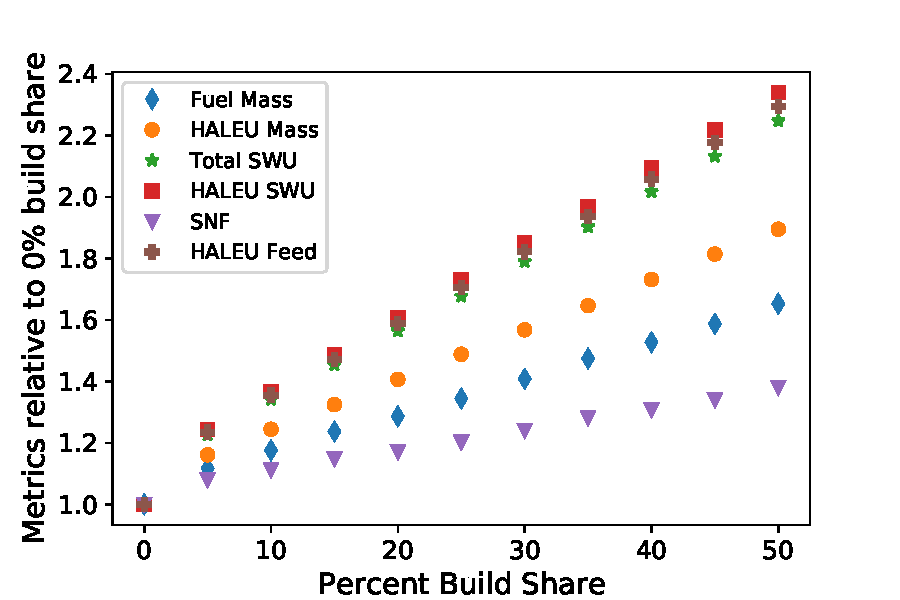
\includegraphics[scale=0.23]{mmr.pdf}
            \caption{Relative effect of varying MMR build share}
            \label{fig:mmr_effects}
    \end{figure}

\end{columns}
\end{frame}

\begin{frame}
    \frametitle{Effects of varying MMR build share}
    \begin{figure}
        \centering
        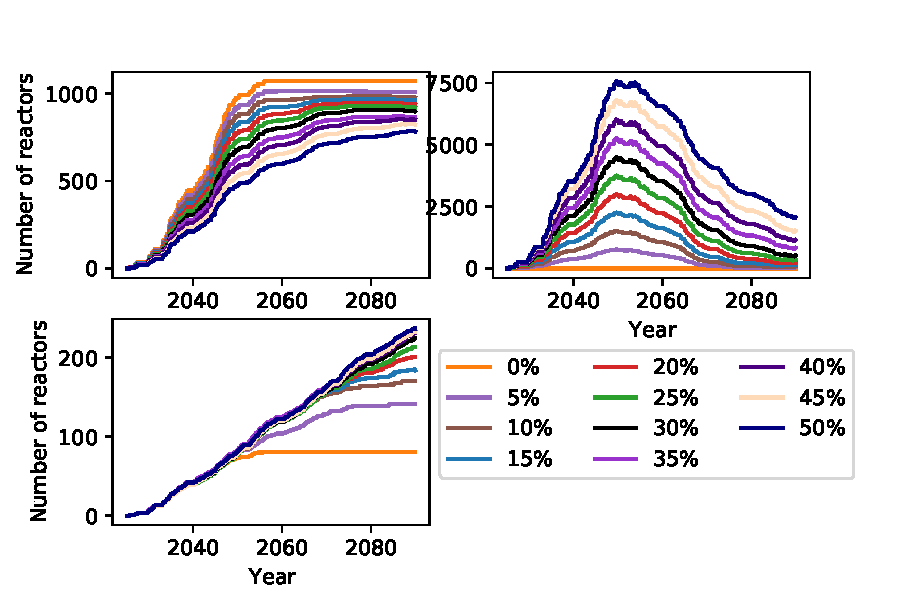
\includegraphics[scale=0.5]{mmr_combined_reactors.pdf}
        \caption{Number of Xe-100s (top left), MMRs (top right), and VOYGRs
        (bottom left) as a function of MMR build share.}
        \label{fig:mmr_s7_combined_reactors}
    \end{figure}
\end{frame}

\begin{frame}
    \frametitle{Effects of varying Xe-100 burnup and MMR build share}
    \begin{columns}

        \column[t]{4cm}
        \begin{itemize}
            \item Non-uniform relationship
            \item At smaller Xe-100 burnup values the increasing MMR 
                  share decreases the HALEU mass
            \item At larger Xe-100 burnup values the increasing MMR share 
                  increases the HALEU mass
            \item Comparison of how much fuel each reactor needs
        \end{itemize}

    \column[t]{6cm}
    \vspace{-1cm}
    \begin{figure}
        \centering 
            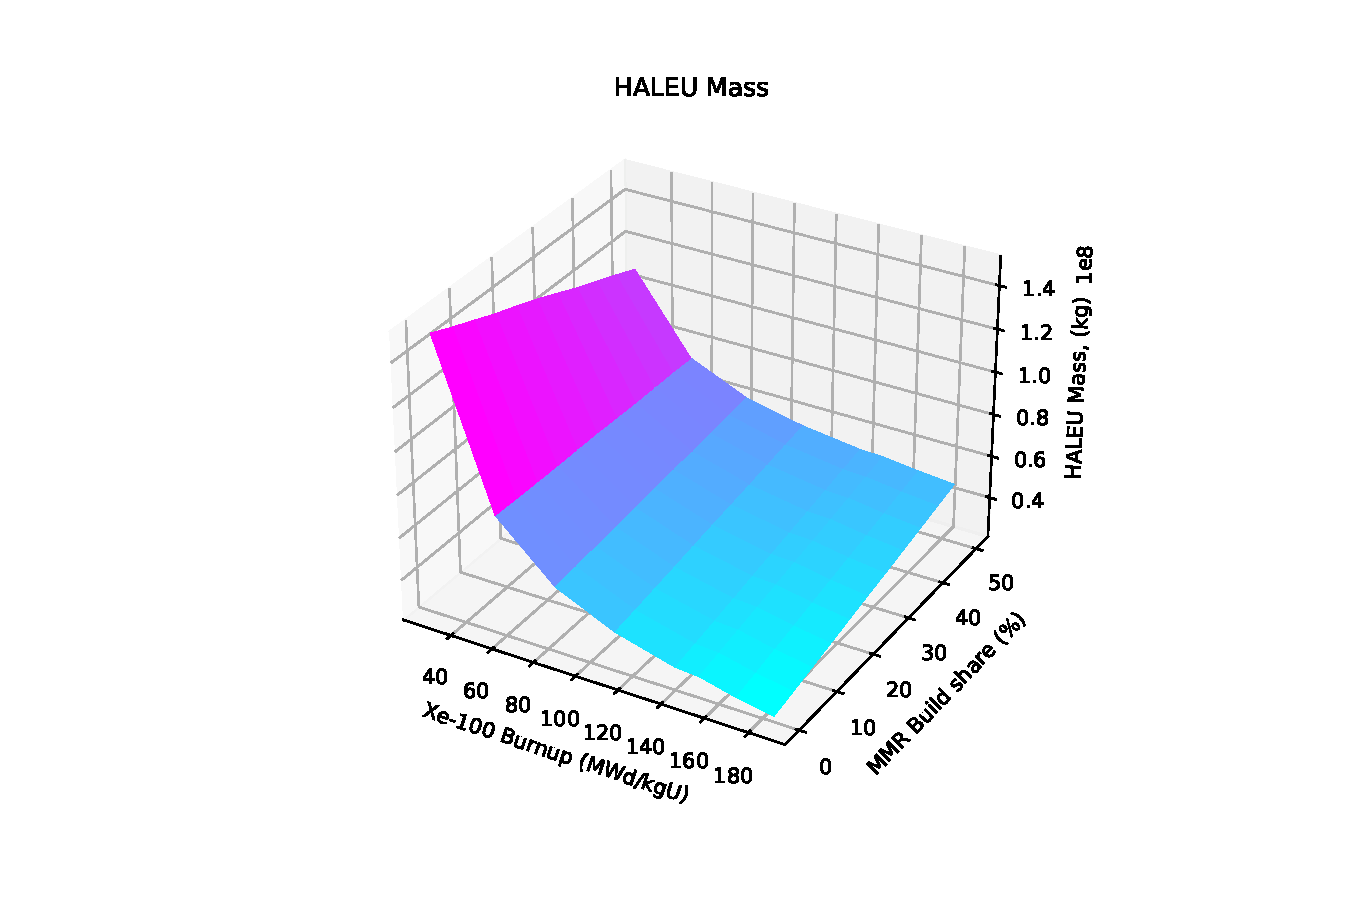
\includegraphics[scale=0.5, trim=180 45 70 50,clip]{mmr_share_xe100_burnup_haleu.pdf}
            \caption{Effects of varying the Xe-100 burnup and MMR build 
            share on HALEU mass requirements. }
            \label{fig:mmr_share_xe100_bu}
    \end{figure}

\end{columns}
\end{frame}

\begin{frame}
    \frametitle{Varying multiple parameters shows importance of the 
    Xe-100 burnup}
    \begin{table}[h!]
        \centering
        \caption{Sobol' indices for the Gaussian model when varying the MMR 
        build share. Highlighted 
        values indicate a total Sobol' indices of above 0.5.}
        \label{tab:s7_sobol_mmr_gaussian}
        \begin{tabular}{c c c c c c c }
            \hline
            & \multicolumn{6}{c}{Output Metric} \\
            Parameter & Fuel & HALEU & SWU & HALEU SWU & Feed & SNF\\
            \hline
            Transition Start & 0.006 & 0.004 & 0.001 &
                               0.001 & 0.001 & 0.006\\
            LWR Lifetime & 0.068 & 0.063 & 0.071 &
                           0.069 & 0.069 & 0.071\\
            MMR Share & 0.107 & 0.107 & 0.203 &
                              0.204 & 0.193 & 0.055\\
            Xe-100 Burnup & \cellcolor{green!25}0.846 & \cellcolor{green!25}0.858 & \cellcolor{green!25}0.732 &
            \cellcolor{green!25}0.734 & \cellcolor{green!25}0.747 & \cellcolor{green!25}0.900\\
            MMR Burnup & 0.049 & 0.050 & 0.071 &
                         0.071 & 0.069 & 0.053\\
            \hline        
        \end{tabular}
    \end{table}
\end{frame}

\subsection{Optimization}
\begin{frame}
    \frametitle{Use the \Cyclus-Dakota coupling to optimize the transition}
    \begin{itemize}
        \item Use the genetic algorithms in Dakota to perform optimization.
        \item Consider the same input parameters as the sensitivity analysis, 
              except the transition start time
        \item<2-> Apply a linear constraint for the advanced reactor build shares
        \item<3-> Goal is to minimize the SWU capacity needed to 
             produce HALEU, the mass of SNF, or both in a multi-objective 
             problem
    \end{itemize}
\end{frame}

\begin{frame}
    \frametitle{Single-objective optimization isn't perfect}
    \begin{columns}
        \column[t]{5cm}
        \begin{itemize}
            \item Maximize Xe-100 build share, LWR lifetimes,
                  and Xe-100 burnup to minimize \gls{SNF} mass
            \item Find a solution that has less SNF mass than the 
                  transition scenarios and the OAT analysis
            \item<2-> Genetic algorithm struggles with linear constraint for 
                  the three build shares
            \item<3-> Results provide guidance, but should explore 
                  other optimization algorithms
        \end{itemize}

        \column[t]{5.5cm}
        \begin{table}[h!]
            \centering 
            \caption{Values resulting in a minimum waste mass disposed of for 
                      a once-through transition scenario.}
            \label{tab:soga_ot_waste}
            \vspace{-0.5cm}
            \begin{tabular}{c c}
                \hline
                Variable & Value \\
                \hline
                LWR Lifetime & 50\%\\
                Xe-100 build share & 100\%\\
                MMR build share & 7\%\\
                VOYGR build share & 11\%\\
                Xe-100 burnup & 185 MWd/kgU\\
                MMR burnup & 90 MWd/kgU\\
                \hline
                SNF mass & 1,736 MT \\
                \hline
            \end{tabular}
        \end{table}
    \end{columns}
    
\end{frame}